\documentclass{tufte-handout}
\usepackage{amsmath,amsthm}

\input{vc.tex}

\usepackage{booktabs}
\usepackage{graphicx}
\usepackage[separate-uncertainty]{siunitx}
\usepackage{tikz}

\newtheorem{claim}{Claim}[section]
\title{\sf Marking Trees}
\date{}
\begin{document}
\maketitle
\footnotetext{\GITAuthorDate, rev. \GITAbrHash}

\begin{marginfigure}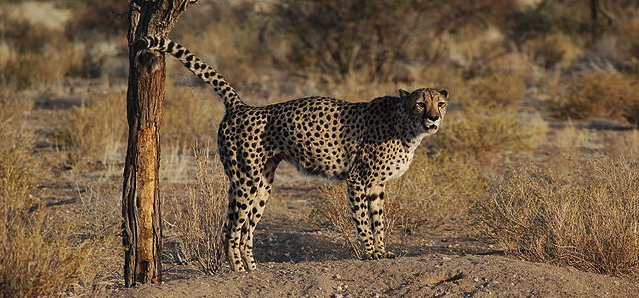
\includegraphics[width=4.5cm]{long_cheetah.png}
\end{marginfigure}

  \medskip\noindent Bob maintains a complete binary tree of height
  $h>1$ with $N=2^h-1$ nodes called $1,\ldots, N$.
  Nodes are in one of two states: marked or unmarked; initially, all
  nodes are unmarked.
  Each round Alice sends an integer $i\in \{1,\ldots, N\}$ according
  to a random process specified below.
  Bob marks node $i$ in his tree.
  Bob then uses the following marking rules repeatedly:
\begin{enumerate}
\item An internal node gets marked when both its children are marked,
  so $\vcenter{\hbox{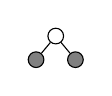
\begin{tikzpicture}[inner sep = 2pt, every
        node/.style={draw,circle}] \node[fill=gray] (u) at (0,0) { };
        \node[fill=gray] (v) at (.5,0) { }; \node (w) at (.25,.3) { };

  \draw[-] (w) edge (u);
  \draw[-] (w) edge (v);
\end{tikzpicture}}}$
becomes
$\vcenter{\hbox{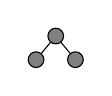
\begin{tikzpicture}[inner sep = 2pt, every node/.style={draw,circle}]
  \node[fill=gray] (u) at (0,0) { };
  \node[fill=gray] (v) at (.5,0) {  };
  \node[fill=gray] (w) at (.25,.3) {  };

  \draw[-] (w) edge (u);
  \draw[-] (w) edge (v);
\end{tikzpicture}}}$.

\item A non-root node gets marked if its parent and sibling are
  marked, so
$\vcenter{\hbox{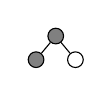
\begin{tikzpicture}[inner sep = 2pt, every node/.style={draw,circle}]
  \node[fill=gray] (u) at (0,0) { };
  \node (v) at (.5,0) {  };
  \node[fill=gray] (w) at (.25,.3) {  };

  \draw[-] (w) edge (u);
  \draw[-] (w) edge (v);
\end{tikzpicture}}}$
becomes
$\vcenter{\hbox{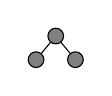
\begin{tikzpicture}[inner sep = 2pt,every node/.style={draw,circle}]
  \node[fill=gray] (u) at (0,0) { };
  \node[fill=gray] (v) at (.5,0) {  };
  \node[fill=gray] (w) at (.25,.3) {  };

  \draw[-] (w) edge (u);
  \draw[-] (w) edge (v);
\end{tikzpicture}}}$
and similarly for a left child.
\end{enumerate}
Bob applies these rules as often as possible, often leading to a
cascade of markings.
When no more rules apply, this round ends. 
For instance, if Alice sends ``5'' in the figure to the right then the
entire tree gets marked in this round.
\begin{marginfigure}
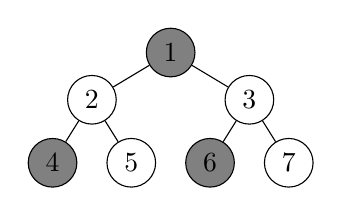
\begin{tikzpicture}[every node/.style={draw,circle}]
  \node (1)[fill=gray] at (1.5,1.4)  { 1 };
  \node (2) at (.5,.8)  { 2 };
  \node (3) at (2.5,.8) { 3 };
  \node (4)[fill=gray] at (0,0) { 4 };
  \node (5) at (1,0) { 5 };
  \node (6)[fill=gray] at (2,0) { 6 };
  \node (7) at (3,0) { 7 };

  \draw[-] (1) edge (2);
  \draw[-] (1) edge (3);
  \draw[-] (2) edge (4);
  \draw[-] (2) edge (5);
  \draw[-] (3) edge (6);
  \draw[-] (3) edge (7);
\end{tikzpicture}
\end{marginfigure}
The whole proces ends when
every node in Bob's tree is marked.



We study 3 random processes:
\begin{enumerate}
\item Each round, Alice sends the name of a node independently and
  uniformly at random from $\{1,\ldots, N\}$.
\item Each round, Alice sends the name of a node uniformly at
  random \emph{from those she has not sent before}.
  Another way of saying this is that Alice starts by picking a random
  permutation $\pi$ on $\{1,\ldots, N\}$ and then sends $\pi(i)$ in
  round $i$.
\item Each round, Alice sends the name of a node uniformly at random
  \emph{from those that are not yet marked}. (Alice can see Bob's tree.)
\end{enumerate}


\emph{Hints:} For $R_2$ and $R_3$, you may be tempted to pick random
numbers uniformly from $\{1,\ldots,N\}$ each round and and throw away
those already sent. That takes too much time.
Instead, for $R_2$ start with a random permutation using the ``Knuth
shuffle''.
Look it up.

To understand what is going on, maybe it helps you to see which nodes
Alice sent. (In particular, what is the last node she sends before the
process stops?)



\newpage
\section{Lab Report: Marking Trees}


by Alice Cooper and Bob Marley\sidenote{Complete the report by filling
  in your names and the parts marked $[\ldots]$.
  Remove the sidenotes in your final hand-in.}

\subsection{Results}

For $i\in\{1,2,3\}$, the number of rounds $R_i$ spent until the tree
is completely marked in process $i$ is given in the following table.
The table shows the result of $[\cdots]$ repeated
trails.\footnote{Report your empirical data.
  Give each value as the mean plus/minus one standard deviation.
  Use whatever best practices for reporting data you may have learned;
  here's a crash course that suffices for our purposes: (i) Calculate mean and standard deviation ($m
  = 2.5074$, $s = 0.889341021813$) from a number of repeated
  experiments.
  (ii) Round $s$ to one significant digit ($s = 0.9$).
  (iii) Round $m$ to the decimal place corresponding to the first
  significant digit in $s$ ($m = 2.5$, $s = 0.9$).
  (iv) Report $m\pm s$ ($2.5 \pm 0.9$).
  (v) Use scientific notation.
  Feel free to go to town with graphs and confidence intervals and so
  forth if that makes you happy.}

\medskip\noindent
\begin{tabular}{
    S[table-format = 7]
    S[table-format = 1.1(1)e1]
    S[table-format = 1.1(1)e1]
    S[table-format = 1.1(1)e1]
  } 
% WARNING: This table the (brilliant) siunitx package.
% This allows typesetting of nicely aligned numbers.
% If this is too much to absorb, just use a normal Latex table.
% (Or do the table in another tool, export as PDF, and include it.)
% Or do the whole report in your favourite word processor instead.
\toprule
{ $N$ } & { $R_1$ } & {$R_2$} & {$R_3$} \\\midrule
3 & 2.6\pm 0.9 \\
7 & \\
15 & \\
31 & \\
63 & \\
127 & \\
255 & \\
511 & \\
1023 & 3.2 \pm 0.5 e3\\
$\vdots$ \\
524287 & 3.2 \pm 0.2 e6 \\
1048575 \\\bottomrule
\end{tabular}

\subsection{Analysis}

Our experimental data indicates that $\mathbf E [R_1]$ is [$\ldots$],
while $\mathbf E[R_2]$ [$\cdots$], and $\mathbf E[R_3]$
[$\cdots$].\footnote{For each of the tree processes, try to express
  the observed behaviour of $R_i$ using standard terminology from the
  analys of algorithms.
  For instance, use expressions such as ``$E[R_1]$ is logarithmic in
  $N$'' or ``$E[R_2]$ is somewhere between $\Omega(N^{1/2})$ and
  $\Omega(N^{3/2})$''.}

Theoretically, the behaviour of $R_1$ can be explained as follows: [$\cdots$] \footnote{This
  is the difficult part.
  You need to write a few lines that explain the random process
  underlying $R_1$ and derive an expression for $\mathbf E[R_1]$.
  (Hopefully it's the same as your empirical analysis!)
  Once you recognize what's going on, this should be easy; it involves
  no complicated calculations.
  Optionally, you can explain the behaviours of $R_2$ and $R_3$ as
  well.
  The behaviour of $R_2$ is quite a bit harder; while $R_3$ is just
  cute.
}



\newpage
\section{Perspective}

This lab establishes minimal skills in simulation of random processes,
introduces the Knuth shuffle for those who haven't seen it, and some
basic probability theory about occupancy problems.
In process 2, Alice's messages are not independent, which can lead to
temping errors in the analysis.
Process 3 is just surprising (and maybe fun to implement), but not
much about randomness is to be learned from it.

The exercise is built on an assigment of Michael
Mitzenmacher.\sidenote{Michael Mitzenmacher, An Experimental
  Assignment on Random Processes, SIGACT News, 27 December 2000.
  See also section 5.8 in M.
  Mitzenmacher and E.
  Upfal, Probability and Computing -- Randomized Algorithms and
  Probabilistic Analysis.
  Cambridge University Press, 2005.}

The front page image shows \emph{Acinonyx jubatus} marking a
tree. Photo by Joachim Huber, under the Creative Commons Attribution-Share
Alike 2.0 Generic license.\sidenote{commons.wikimedia.org/\-wiki/\-File:\-Acinonyx\_jubatus\_-\-Southern\_Namibia-8.jpg}

\end{document}
